\documentclass[11pt,a4paper]{article}

\usepackage[utf8]{inputenc}
\usepackage[T1]{fontenc}
\usepackage[french]{babel}
\usepackage{lmodern}
\usepackage[margin=2.5cm]{geometry}
\usepackage{amsmath}
\usepackage{graphicx}
\usepackage{subcaption}
\usepackage{booktabs}
\usepackage{array}
\usepackage{float}
\usepackage{listings}
\usepackage{xcolor}
\usepackage[hidelinks]{hyperref}

% Les figures sont celles generees par nos scripts
\graphicspath{{../figures/}}

% Autorise un retour a la ligne apres les _ des noms de fichiers
\let\underscoreorig\_
\renewcommand{\_}{\underscoreorig\allowbreak}
\emergencystretch=1em

\lstset{
  basicstyle=\ttfamily\small,
  columns=fullflexible,
  keepspaces=true,
  frame=single,
  breaklines=true,
}

\title{TD Clustering -- Compte rendu}
\author{NGUYEN Dinh Huy \and NGUYEN Vinh Tri}
\date{Data Mining -- INSA Centre Val de Loire -- Novembre 2026}

\begin{document}

\maketitle
\tableofcontents

% ======================================================================
\section*{Organisation du rendu et utilisation du code}
\addcontentsline{toc}{section}{Organisation du rendu et utilisation du code}

L'archive contient :
\begin{itemize}
  \item \texttt{section1\_kmeans.py} : notre k-means (Section 1, Exercices 1 à 3) ;
  \item \texttt{section1\_sklearn.py} : la comparaison avec SciKit-Learn (Section 1, Exercice 4) ;
  \item \texttt{section1\_verifications.py} : la comparaison de notre affichage avec celui de l'énoncé (Section 1, Exercice 1) ;
  \item \texttt{section2\_hierarchique.py} : le clustering hiérarchique (Section 2) ;
  \item \texttt{section3\_etude\_de\_cas.py} : l'étude de cas (Section 3) ;
  \item \texttt{data/Country-data.csv} : le jeu de données de l'étude de cas ;
  \item \texttt{figures/} : les figures générées par les scripts ;
  \item \texttt{requirements.txt}, \texttt{README.md}, et \texttt{rapport/} qui contient ce compte rendu et son source LaTeX.
\end{itemize}

\paragraph{Installation.} Notre distribution Linux n'autorise pas \texttt{pip install} en dehors d'un environnement virtuel, nous avons donc installé les bibliothèques ainsi :
\begin{lstlisting}
python3 -m venv .venv
.venv/bin/pip install -r requirements.txt
\end{lstlisting}

\paragraph{Exécution.} Depuis la racine du projet :
\begin{center}
\begin{tabular}{@{}ll@{}}
  \toprule
  Commande & Résultat \\
  \midrule
  \texttt{.venv/bin/python section1\_kmeans.py} & Exercices 1 à 3, figures \texttt{ex3\_*.png} \\
  \texttt{.venv/bin/python section1\_sklearn.py} & Exercice 4 \\
  \texttt{.venv/bin/python section1\_verifications.py} & Vérification de l'Exercice 1 \\
  \texttt{.venv/bin/python section2\_hierarchique.py} & Section 2, figures \texttt{s2\_*.png} \\
  \texttt{.venv/bin/python section3\_etude\_de\_cas.py} & Section 3, figures \texttt{s3\_*.png} \\
  \bottomrule
\end{tabular}
\end{center}
Chaque script affiche les résultats cités dans ce compte rendu. Les tirages aléatoires de la Section 3 utilisent une graine fixe, donc les résultats et les figures sont les mêmes à chaque exécution.

% ======================================================================
\section{Clustering k-means}

\subsection{Exercice 1 : implémentation de k-means}

Notre implémentation est dans \texttt{section1\_kmeans.py} et n'utilise que les modules \texttt{math} et \texttt{random} (Matplotlib sert seulement aux figures de l'Exercice 3). Un point est une liste de nombres (\texttt{[1]} en 1D, \texttt{[-2, 3]} en 2D) et tous les calculs se font coordonnée par coordonnée, donc le code marche quelle que soit la dimension.
\begin{lstlisting}
kmeans(data, k, centroides_initiaux=None)
\end{lstlisting}
La fonction affiche les résultats intermédiaires et retourne la SSE. Elle procède ainsi :
\begin{enumerate}
  \item \textbf{Initialisation} : si \texttt{centroides\_initiaux} vaut \texttt{None}, on tire $k$ points du jeu de données au hasard (\texttt{random.sample}).
  \item \textbf{Affectation} : chaque point va au centroïde le plus proche (distance euclidienne). En cas d'égalité, il va au centroïde de plus petit indice.
  \item \textbf{Mise à jour} : chaque centroïde devient la moyenne des points de son cluster. Un cluster vide garde son ancien centroïde.
  \item \textbf{Arrêt} : on recommence les étapes 2 et 3 jusqu'à ce que l'affectation ne change plus.
  \item \textbf{Erreur} : on retourne $\mathrm{SSE} = \sum_{j=1}^{k} \sum_{x \in C_j} d(x, c_j)^2$.
\end{enumerate}

Pour vérifier l'affichage, \texttt{section1\_verifications.py} compare la sortie de notre fonction avec le texte de l'énoncé pour les deux exemples : elle est identique (SSE de 98.0 et de 2.5).

\subsection{Exercice 2 : tests sur le jeu de données [[2], [4], [6], [12], [24], [30]]}

\medskip\noindent\textbf{(a) Centroïdes initiaux \texttt{[[2], [6]]}}
\begin{lstlisting}
Iteration 1
Centroid [2]  Points [[2], [4]]
Centroid [6]  Points [[6], [12], [24], [30]]
Iteration 2
Centroid [3.0]  Points [[2], [4], [6]]
Centroid [18.0]  Points [[12], [24], [30]]
Iteration 3
Centroid [4.0]  Points [[2], [4], [6], [12]]
Centroid [22.0]  Points [[24], [30]]
Iteration 4
Centroid [6.0]  Points [[2], [4], [6], [12]]
Centroid [27.0]  Points [[24], [30]]
Fin clustering, erreur =  74.0
\end{lstlisting}

\medskip\noindent\textbf{(b) Centroïdes initiaux \texttt{[[12], [24]]}}
\begin{lstlisting}
Iteration 1
Centroid [12]  Points [[2], [4], [6], [12]]
Centroid [24]  Points [[24], [30]]
Iteration 2
Centroid [6.0]  Points [[2], [4], [6], [12]]
Centroid [27.0]  Points [[24], [30]]
Fin clustering, erreur =  74.0
\end{lstlisting}

\paragraph{Discussion.} Les deux initialisations donnent le même clustering, $\{2, 4, 6, 12\}$ et $\{24, 30\}$, avec la même SSE (74.0) : aucune n'est meilleure que l'autre. Seul le nombre d'itérations change. Avec (b), les centroïdes 12 et 24 sont déjà de part et d'autre de la séparation, donc le bon clustering est trouvé dès la première itération. Avec (a), les deux centroïdes partent à gauche et le second doit se déplacer vers la droite (6, 18, 22 puis 27), d'où 4 itérations. Au passage, à l'itération 1 de (a), le point 4 est à égale distance de 2 et de 6 : il va dans le premier cluster d'après notre règle.

\subsection{Exercice 3 : visualisations 2D}

Nous avons ajouté trois paramètres optionnels :
\begin{lstlisting}
kmeans(data, k, centroides_initiaux=None, noms=None,
       prefixe_figures=None, retourner_clusters=False)
\end{lstlisting}
\begin{itemize}
  \item \texttt{noms} : les noms des points, dans le même ordre que \texttt{data}, pour les annoter sur les figures ;
  \item \texttt{prefixe\_figures} : si ce paramètre est donné, la figure de l'itération $i$ est sauvegardée dans \texttt{<prefixe\_figures>\_iter<i>.png}. Nous sauvegardons les figures plutôt que de les afficher pour pouvoir les mettre dans le compte rendu ;
  \item \texttt{retourner\_clusters} : si \texttt{True}, la fonction retourne (SSE, clusters finaux) au lieu de la SSE seule. Il sert à l'Exercice 4 et à l'étude de cas.
\end{itemize}
Avec les valeurs par défaut, la fonction se comporte comme à l'Exercice 1. Sur chaque figure, les points sont des $\bullet$ annotés et les centroïdes des $\times$, de la couleur de leur cluster (rouge pour le premier, bleu pour le second). Nous avons pris un cadre de $-4$ à $4$ au lieu de $-3$ à $3$ pour que M1 ne soit pas collé au bord.

Les figures sont générées par \texttt{.venv/bin/python section1\_kmeans.py}, avec ces deux appels (extrait simplifié) :
\begin{lstlisting}
M = [[-2, 3], [-2, 1], [-2, -1], [2, -1], [2, 1], [1, 0]]
noms_M = ["M1", "M2", "M3", "M4", "M5", "M6"]
kmeans(M, 2, [M[0], M[1]], noms=noms_M,
       prefixe_figures="figures/ex3_init_M1_M2")   # M1 et M2
kmeans(M, 2, [M[3], M[5]], noms=noms_M,
       prefixe_figures="figures/ex3_init_M4_M6")   # M4 et M6
\end{lstlisting}

\begin{figure}[H]
  \centering
  \begin{subfigure}{0.32\textwidth}
    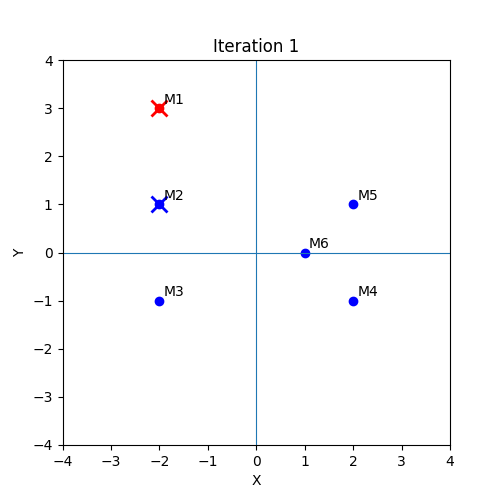
\includegraphics[width=\linewidth]{ex3_init_M1_M2_iter1.png}
    \caption{Itération 1}
  \end{subfigure}
  \begin{subfigure}{0.32\textwidth}
    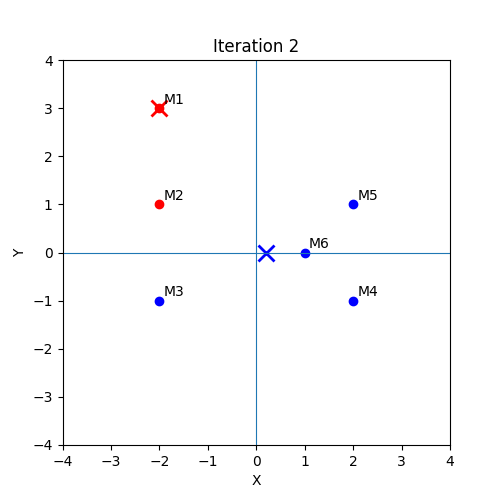
\includegraphics[width=\linewidth]{ex3_init_M1_M2_iter2.png}
    \caption{Itération 2}
  \end{subfigure}
  \begin{subfigure}{0.32\textwidth}
    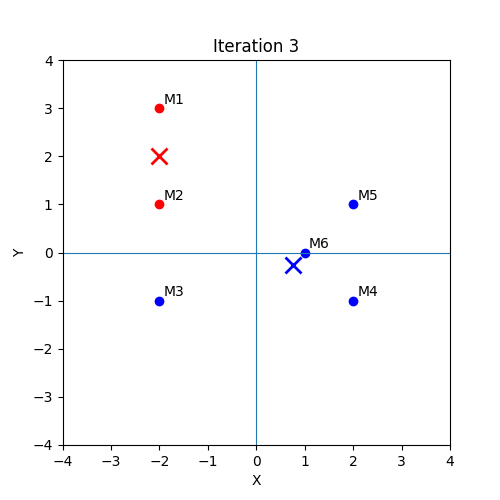
\includegraphics[width=\linewidth]{ex3_init_M1_M2_iter3.png}
    \caption{Itération 3}
  \end{subfigure}
  \caption{Centroïdes initiaux M1 et M2. SSE finale : 15.5.}
  \label{fig:ex3-m1m2}
\end{figure}

\begin{figure}[H]
  \centering
  \begin{subfigure}{0.32\textwidth}
    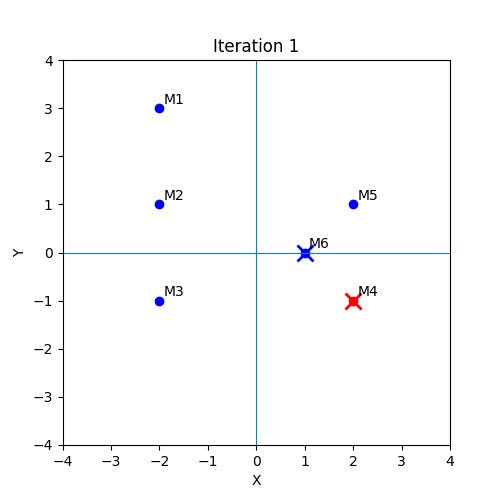
\includegraphics[width=\linewidth]{ex3_init_M4_M6_iter1.png}
    \caption{Itération 1}
  \end{subfigure}
  \begin{subfigure}{0.32\textwidth}
    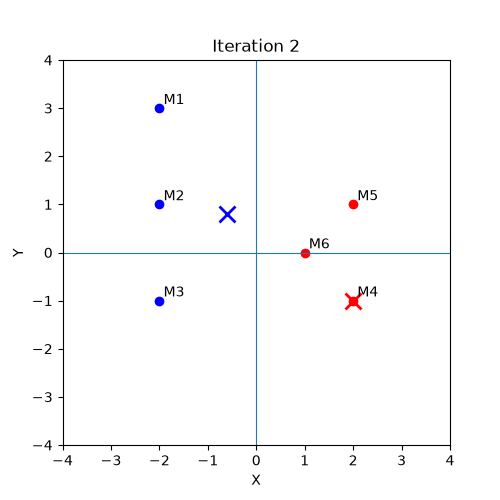
\includegraphics[width=\linewidth]{ex3_init_M4_M6_iter2.png}
    \caption{Itération 2}
  \end{subfigure}
  \begin{subfigure}{0.32\textwidth}
    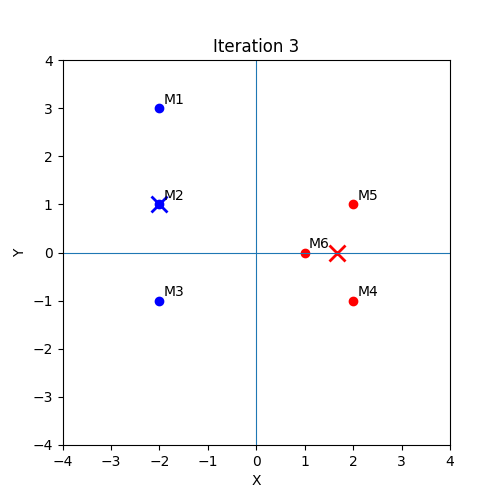
\includegraphics[width=\linewidth]{ex3_init_M4_M6_iter3.png}
    \caption{Itération 3}
  \end{subfigure}
  \caption{Centroïdes initiaux M4 et M6. SSE finale : 10.67.}
  \label{fig:ex3-m4m6}
\end{figure}

Nous obtenons les mêmes séquences que dans l'énoncé.

\subsection{Exercice 4 : comparaison avec SciKit-Learn}

\texttt{section1\_sklearn.py} lance d'abord le code de l'énoncé, qui affiche bien \texttt{[0 1 2 2 2]} et \texttt{[0 0 1 1 2]}.

\paragraph{Pourquoi ce sont les clusters de l'Exercice 1.} \texttt{labels\_} donne le numéro du cluster de chaque point de \texttt{data1}, dans l'ordre. Deux points sont dans le même cluster s'ils ont le même numéro. \texttt{[0 1 2 2 2]} correspond donc à \{1\}, \{2\}, \{18, 20, 31\}, le résultat obtenu avec \texttt{[[1], [2], [18]]}, et \texttt{[0 0 1 1 2]} à \{1, 2\}, \{18, 20\}, \{31\}, obtenu avec \texttt{[[18], [20], [31]]}. Les numéros eux-mêmes n'ont pas d'importance, seul compte quels points ont le même.

\paragraph{Exercices 2 et 3.} Le script refait ensuite tous les clusterings avec \texttt{KMeans(n\_clusters=k, n\_init=1, init=array(...))} et les compare aux nôtres, sans tenir compte de la numérotation des clusters. Il compare aussi notre SSE à \texttt{inertia\_} (avec \texttt{math.isclose}, à cause des arrondis).
\begin{center}
\begin{tabular}{@{}llccc@{}}
  \toprule
  Exercice & Centroïdes initiaux & SSE & Mêmes clusters & Même SSE \\
  \midrule
  1 & \texttt{[[1], [2], [18]]}   & 98.0  & OUI & OUI \\
  1 & \texttt{[[18], [20], [31]]} & 2.5   & OUI & OUI \\
  2 (a) & \texttt{[[2], [6]]}     & 74.0  & OUI & OUI \\
  2 (b) & \texttt{[[12], [24]]}   & 74.0  & OUI & OUI \\
  3 & M1, M2                      & 15.5  & OUI & OUI \\
  3 & M4, M6                      & 10.67 & OUI & OUI \\
  \bottomrule
\end{tabular}
\end{center}
SciKit-Learn trouve les mêmes clusters que nous dans les six cas.

% ======================================================================
\section{Clustering hiérarchique}

Le code est dans \texttt{section2\_hierarchique.py}. La fonction \texttt{dendrogramme} lance le clustering avec \texttt{linkage} (méthode \texttt{"single"} ou \texttt{"complete"}) puis dessine le dendrogramme avec \texttt{dendrogram}, deux fonctions de \texttt{scipy.cluster.hierarchy}. La fonction \texttt{figure\_single\_complete} met les deux dendrogrammes côte à côte et sauvegarde la figure. Le script affiche aussi les fusions successives.

\subsection{Matrice de distance}

La matrice est donnée à \texttt{linkage} au format compact 1D, c'est-à-dire les valeurs au-dessus de la diagonale lues ligne par ligne :
\begin{lstlisting}
data = [0.1, 0.9, 0.35, 0.8, 0.3, 0.4, 0.5, 0.6, 0.7, 0.2]
\end{lstlisting}

\begin{figure}[H]
  \centering
  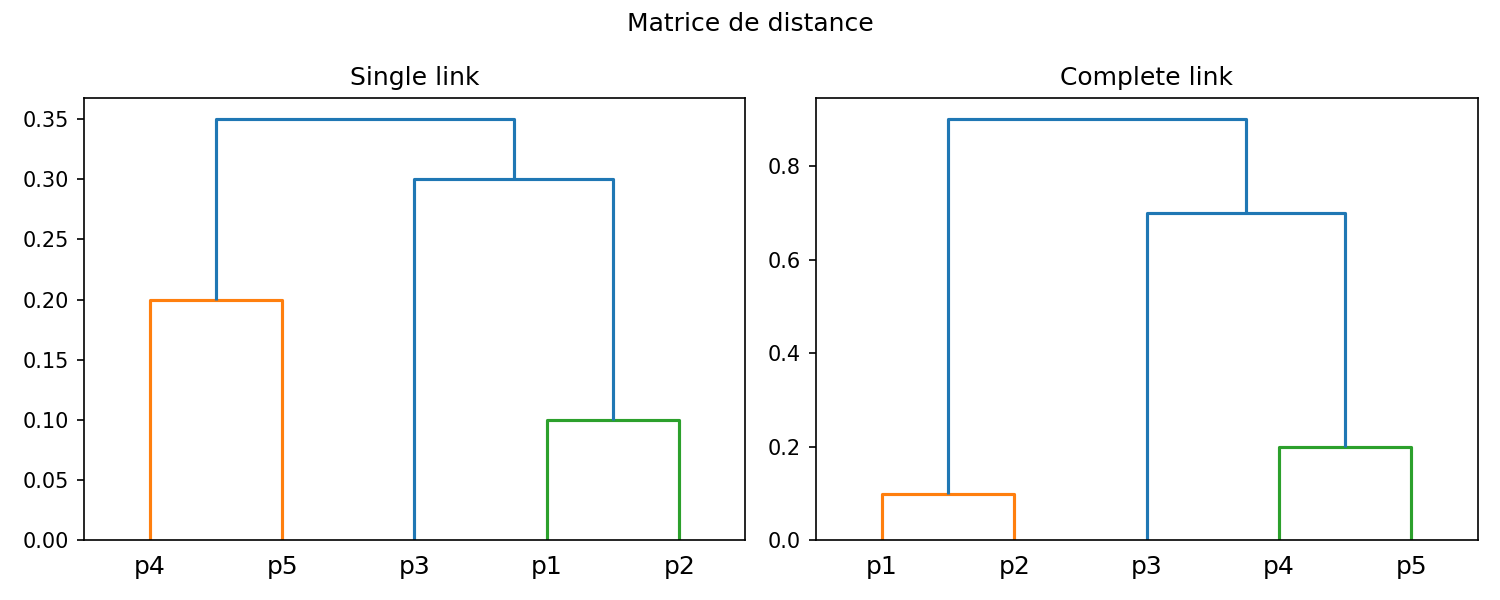
\includegraphics[width=\textwidth]{s2_distance.png}
  \caption{Dendrogrammes obtenus avec la matrice de distance.}
  \label{fig:s2-distance}
\end{figure}

Nous obtenons les mêmes dendrogrammes que l'énoncé. Les deux premières fusions sont identiques dans les deux méthodes ($\{p_1, p_2\}$ à 0.1, puis $\{p_4, p_5\}$ à 0.2), car entre deux points seuls il n'y a qu'une distance possible. La différence vient de $p_3$ :
\begin{itemize}
  \item en single link, la distance entre deux clusters est la plus petite distance entre leurs points. $p_3$ est à $\min(0.9, 0.3) = 0.3$ de $\{p_1, p_2\}$ et à $\min(0.6, 0.7) = 0.6$ de $\{p_4, p_5\}$, il rejoint donc $\{p_1, p_2\}$ ;
  \item en complete link, c'est la plus grande distance : $\max(0.9, 0.3) = 0.9$ contre $\max(0.6, 0.7) = 0.7$, donc $p_3$ rejoint $\{p_4, p_5\}$.
\end{itemize}
Pour la même raison, la dernière fusion se fait à 0.35 en single link ($d(p_1, p_4)$, la plus petite distance entre les deux groupes) et à 0.9 en complete link ($d(p_1, p_3)$, la plus grande).

\subsection{Matrice de similarité}

Il faut d'abord convertir la similarité en distance avec $\mathrm{distance} = 1 - \mathrm{similarit\acute{e}}$. Nous calculons \texttt{1 - sim} sur la matrice $5 \times 5$, puis \texttt{squareform} (de \texttt{scipy.spatial.distance}) la met au format compact. Nous avons choisi \texttt{squareform} parce qu'elle vérifie en plus que la matrice est symétrique avec une diagonale nulle, ce qui détecte une erreur de recopie. On obtient :
\begin{lstlisting}
[0.9, 0.59, 0.45, 0.65, 0.36, 0.53, 0.02, 0.56, 0.15, 0.24]
\end{lstlisting}

\begin{figure}[H]
  \centering
  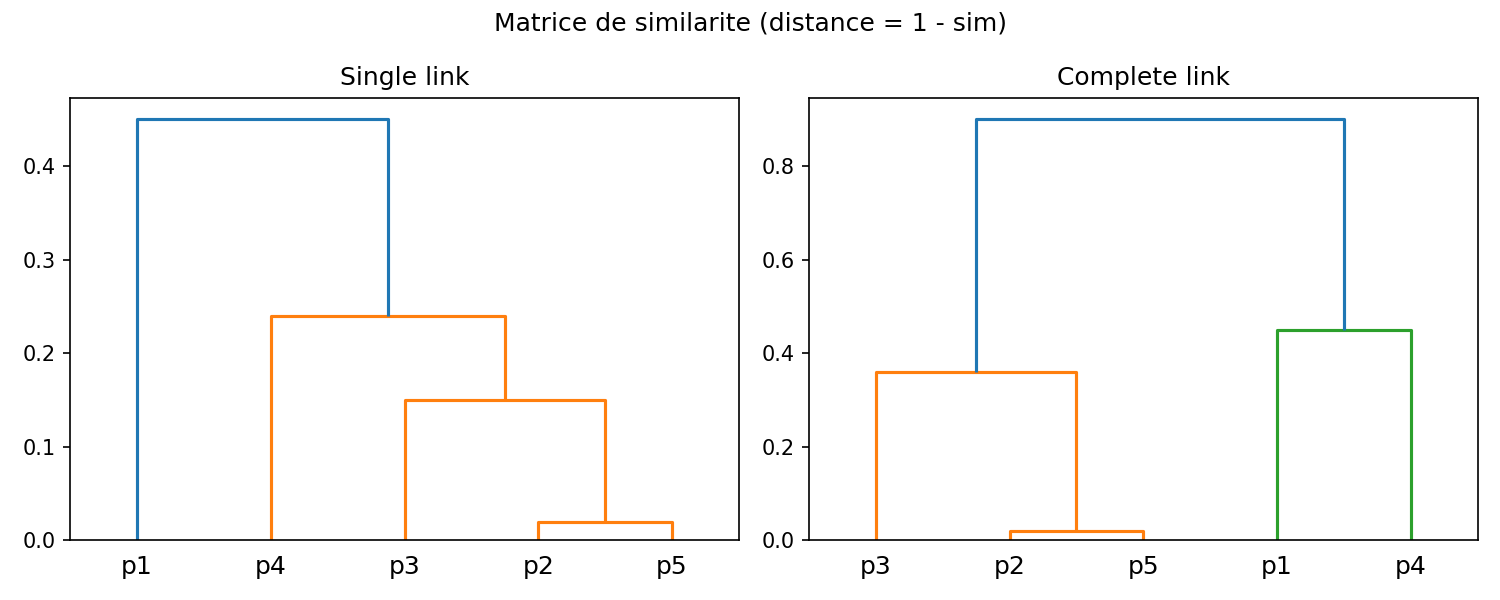
\includegraphics[width=\textwidth]{s2_similarite.png}
  \caption{Dendrogrammes obtenus avec la matrice de similarité convertie en distances.}
  \label{fig:s2-similarite}
\end{figure}

Nous obtenons aussi les dendrogrammes de l'énoncé. En single link, $p_2$ et $p_5$ fusionnent d'abord (0.02), puis $p_3$ (0.15), $p_4$ (0.24) et enfin $p_1$ (0.45) rejoignent ce cluster un par un. C'est l'effet de chaîne du single link : il suffit d'être proche d'un seul point du cluster pour y entrer. Par exemple, $p_4$ entre grâce à $d(p_4, p_5) = 0.24$, alors qu'il est à 0.53 de $p_2$ et à 0.56 de $p_3$. En complete link, $p_4$ est à 0.56 de ce cluster (sa plus grande distance), donc il se regroupe plutôt avec $p_1$ (0.45). On obtient deux groupes plus compacts, $\{p_2, p_3, p_5\}$ et $\{p_1, p_4\}$, qui ne fusionnent qu'à 0.9.

% ======================================================================
\section{Étude de cas}

Le code est dans \texttt{section3\_etude\_de\_cas.py}.

\subsection{Exercice 1 : préparation des données}

\paragraph{Lecture du fichier.} La fonction \texttt{lire\_donnees} retourne la liste \texttt{countries} des 167 noms de pays (pour étiqueter les figures) et la liste \texttt{data\_country} de 167 listes de 9 nombres. Nous utilisons le module \texttt{csv} et non un simple \texttt{split(",")}, car quatre noms de pays contiennent une virgule et sont entre guillemets dans le fichier (par exemple \texttt{"Congo, Dem. Rep."}). Le script affiche le début de \texttt{data\_country}, qui est bien celui de l'énoncé :
\begin{lstlisting}
[[90.2, 10.0, 7.58, 44.9, 1610.0, 9.44, 56.2, 5.82, 553.0],
 [16.6, 28.0, 6.55, 48.6, 9930.0, 4.49, 76.3, 1.65, 4090.0], ...
\end{lstlisting}

\paragraph{ACP.} La fonction \texttt{preparer\_donnees} reprend le squelette de l'énoncé. Nous avons dû remplacer la ligne \texttt{eigenvectors = eig(R)[1]} par :
\begin{lstlisting}
valeurs_propres, eigenvectors = eig(R)
# 1) R est symetrique reelle : ses valeurs propres sont reelles
assert np.allclose(valeurs_propres.imag, 0) and np.allclose(eigenvectors.imag, 0)
valeurs_propres, eigenvectors = valeurs_propres.real, eigenvectors.real
# 2) eig ne trie pas les valeurs propres : ordre decroissant
ordre = argsort(valeurs_propres)[::-1]
valeurs_propres, eigenvectors = valeurs_propres[ordre], eigenvectors[:, ordre]
# 3) le signe d'un vecteur propre est arbitraire : on prend celui de l'enonce
for c in range(2):
    if matmul(Z[0], eigenvectors[:, c]) * REFERENCE_ENONCE[c] < 0:
        eigenvectors[:, c] = -eigenvectors[:, c]
\end{lstlisting}
\begin{enumerate}
  \item Chez nous, \texttt{eig} renvoie des nombres complexes, avec une partie imaginaire nulle. Nous gardons la partie réelle après avoir vérifié qu'elle est bien nulle.
  \item \texttt{eig} ne range pas forcément les valeurs propres de la plus grande à la plus petite. Nous les trions pour que les colonnes 0 et 1 soient bien les deux composantes principales.
  \item Si $v$ est un vecteur propre, $-v$ aussi, et \texttt{eig} peut renvoyer l'un ou l'autre. Cela retourne la figure mais ne change pas les distances. Nous prenons le signe qui donne le même premier point que l'énoncé, pour avoir des figures orientées comme les siennes.
\end{enumerate}
Le début de \texttt{data\_reduced} est bien celui de l'énoncé : \texttt{[[2.91, -0.1], [-0.43, 0.59], ...]}. Les deux composantes expliquent 46.0\,\% et 17.2\,\% de la variance, soit 63.1\,\% : la projection en 2D perd donc une partie de l'information.

\subsection{Exercice 2 : clustering et interprétation}

\subsubsection*{Clustering k-means}

Nous appliquons la fonction \texttt{kmeans} de la Section 1 à \texttt{data\_reduced}, avec des centroïdes initiaux tirés au hasard. Avec 167 points, l'affichage des itérations est illisible, donc le script le masque et n'affiche qu'un résumé. Pour que le résultat soit reproductible, nous fixons la graine du tirage (\texttt{random.seed}). Nous avons choisi les graines 0 pour $k = 2$ et 13 pour $k = 3$ car elles redonnent les clusterings des Figures 1 et 2 de l'énoncé.

\begin{center}
\begin{tabular}{@{}cccccc@{}}
  \toprule
  $k$ & Graine & Itérations & SSE & Taille des clusters & Figure \\
  \midrule
  2 & 0  & 14 & 503.12 & 89 (rouge), 78 (bleu) & \ref{fig:s3-k2} \\
  3 & 13 & 8  & 373.47 & 41 (rouge), 48 (bleu), 78 (orange) & \ref{fig:s3-k3} \\
  \bottomrule
\end{tabular}
\end{center}

\begin{figure}[p]
  \centering
  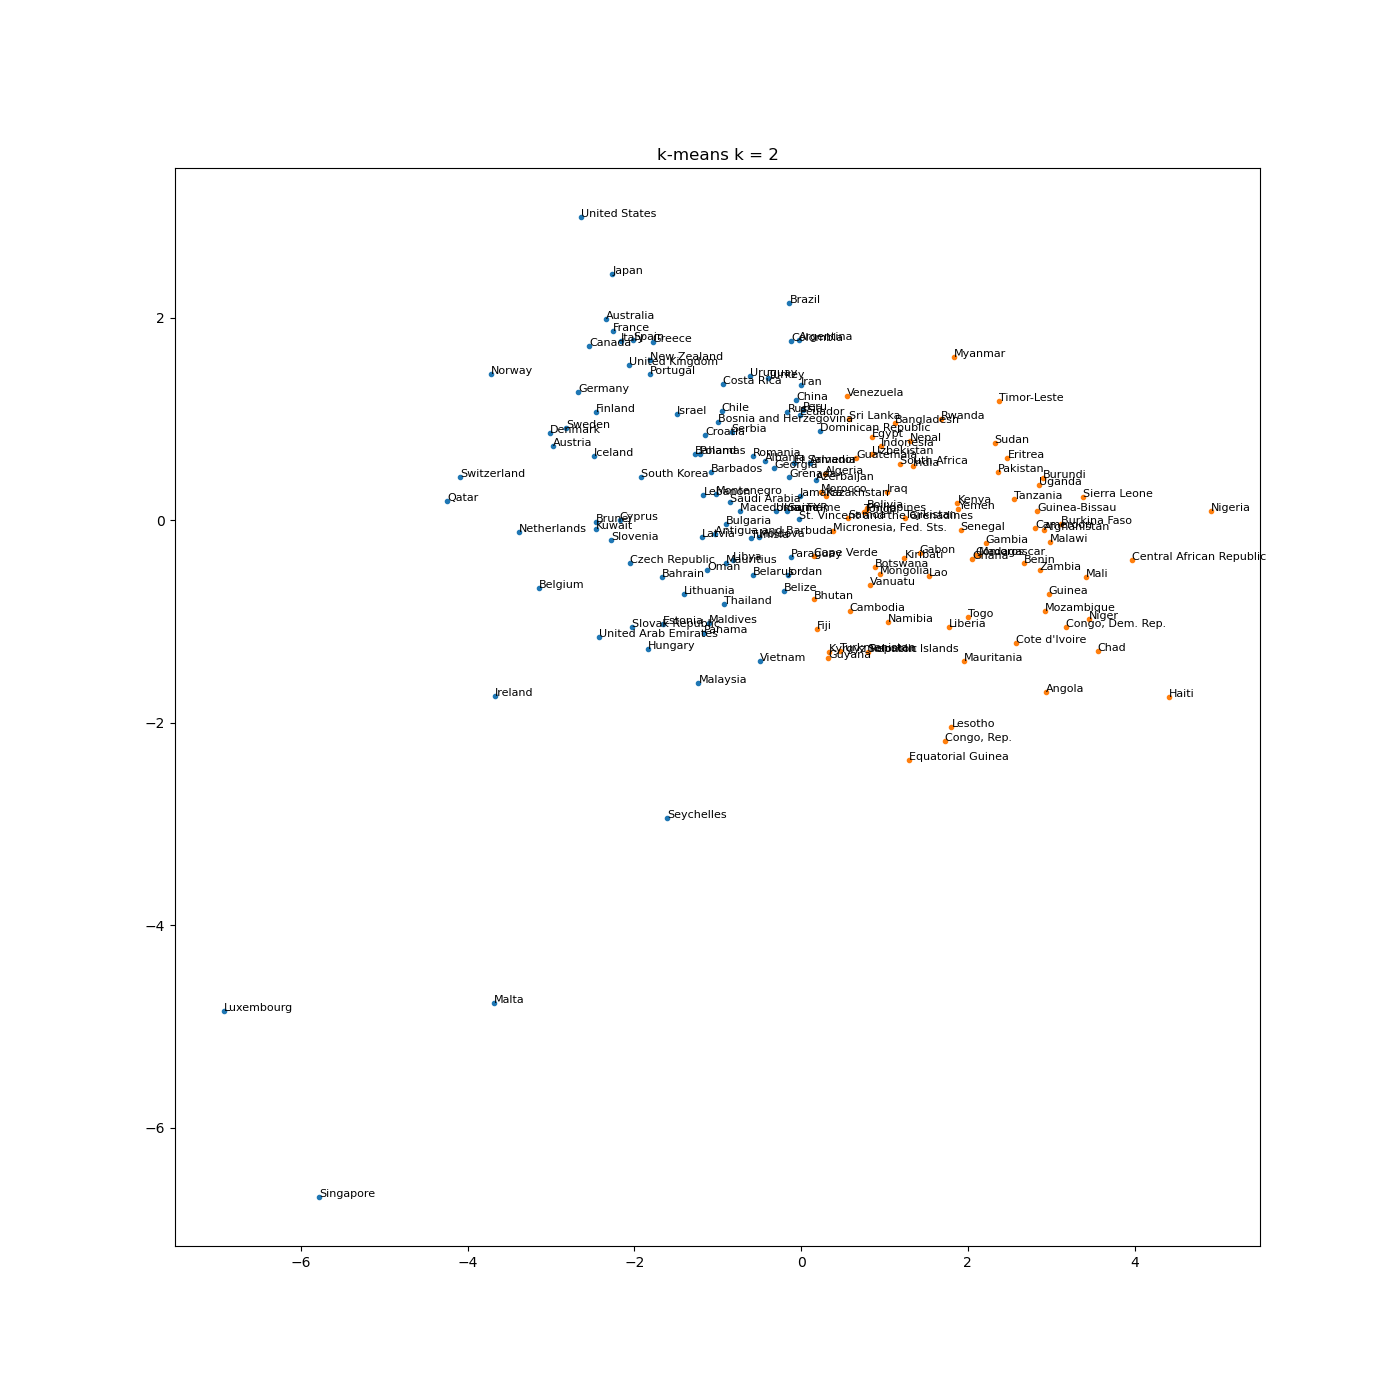
\includegraphics[width=\textwidth,trim=80 60 85 90,clip]{s3_kmeans_k2.png}
  \caption{k-means avec $k = 2$ sur \texttt{data\_reduced}.}
  \label{fig:s3-k2}
\end{figure}

\begin{figure}[p]
  \centering
  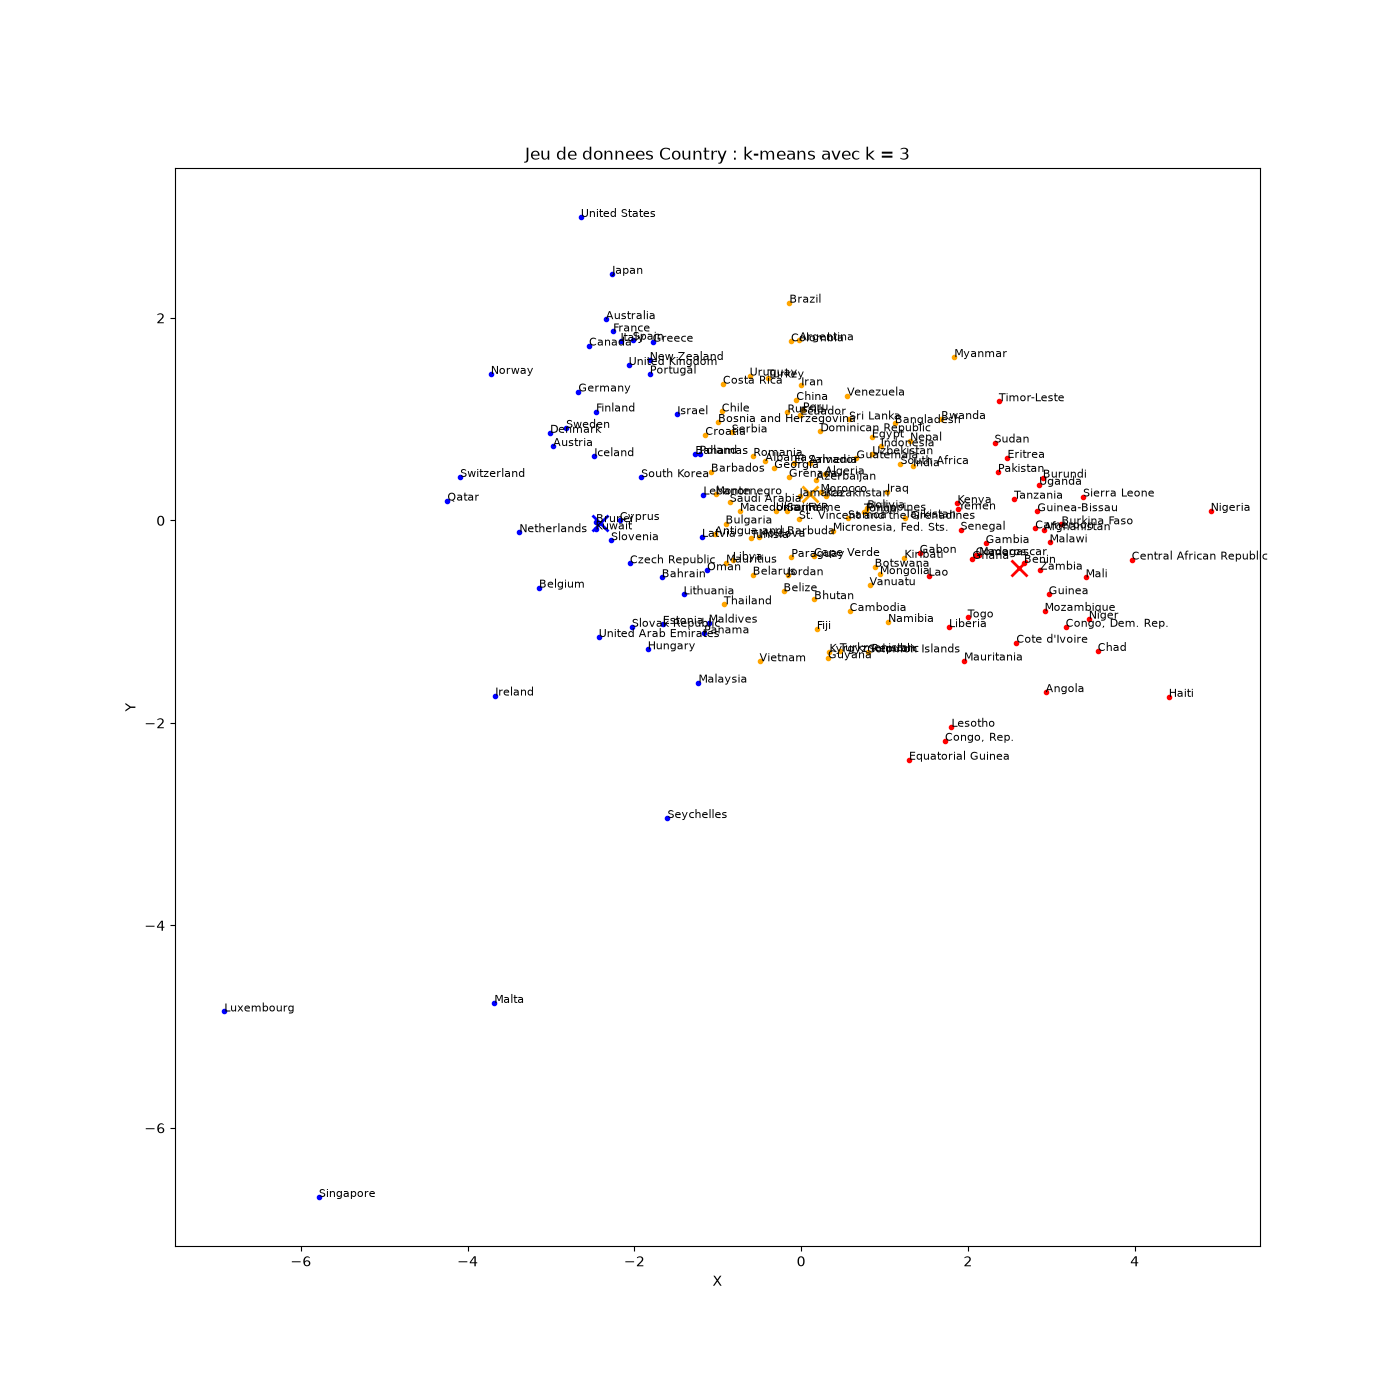
\includegraphics[width=\textwidth,trim=80 60 85 90,clip]{s3_kmeans_k3.png}
  \caption{k-means avec $k = 3$ sur \texttt{data\_reduced}.}
  \label{fig:s3-k3}
\end{figure}

\paragraph{Aurait-on pu obtenir des clusterings très différents ?} Pour le savoir, le script relance k-means avec les graines 0 à 199 et compte les clusterings obtenus :
\begin{center}
\begin{tabular}{@{}cccl@{}}
  \toprule
  $k$ & Tirages & SSE & Clustering obtenu \\
  \midrule
  2 & 107 & 503.12 & celui de la Figure~\ref{fig:s3-k2} \\
  2 & 85  & 503.02 & le même, sauf Azerbaijan et Dominican Republic \\
  2 & 8   & 762.70 & Ireland, Luxembourg, Malta et Singapore seuls \\
  \midrule
  3 & 56  & 373.47 & celui de la Figure~\ref{fig:s3-k3} \\
  3 & 144 & 354.52 à 415.12 & 29 autres clusterings \\
  \bottomrule
\end{tabular}
\end{center}
Pour $k = 2$, le résultat est presque toujours le même. Pour $k = 3$ en revanche, nous obtenons 30 clusterings différents et celui de l'énoncé ne sort que 56 fois sur 200. Certains sont proches (tailles 40, 47 et 80 par exemple), d'autres très différents (23, 70 et 74 pays, ou un cluster qui ne contient que Luxembourg, Malta et Singapore). Donc oui, surtout pour $k = 3$, nous aurions pu obtenir des clusterings assez différents de ceux de l'énoncé.

\subsubsection*{Clustering hiérarchique}

Nous réutilisons la fonction \texttt{dendrogramme} de la Section 2 sans la modifier : avec une liste de points, \texttt{hierarchy.linkage} calcule lui-même les distances euclidiennes. Le dendrogramme est dessiné à l'horizontale pour que les noms des pays restent lisibles. Nous obtenons les mêmes dendrogrammes que les Figures 3 et 4 de l'énoncé (même ordre des pays).

\begin{figure}[p]
  \centering
  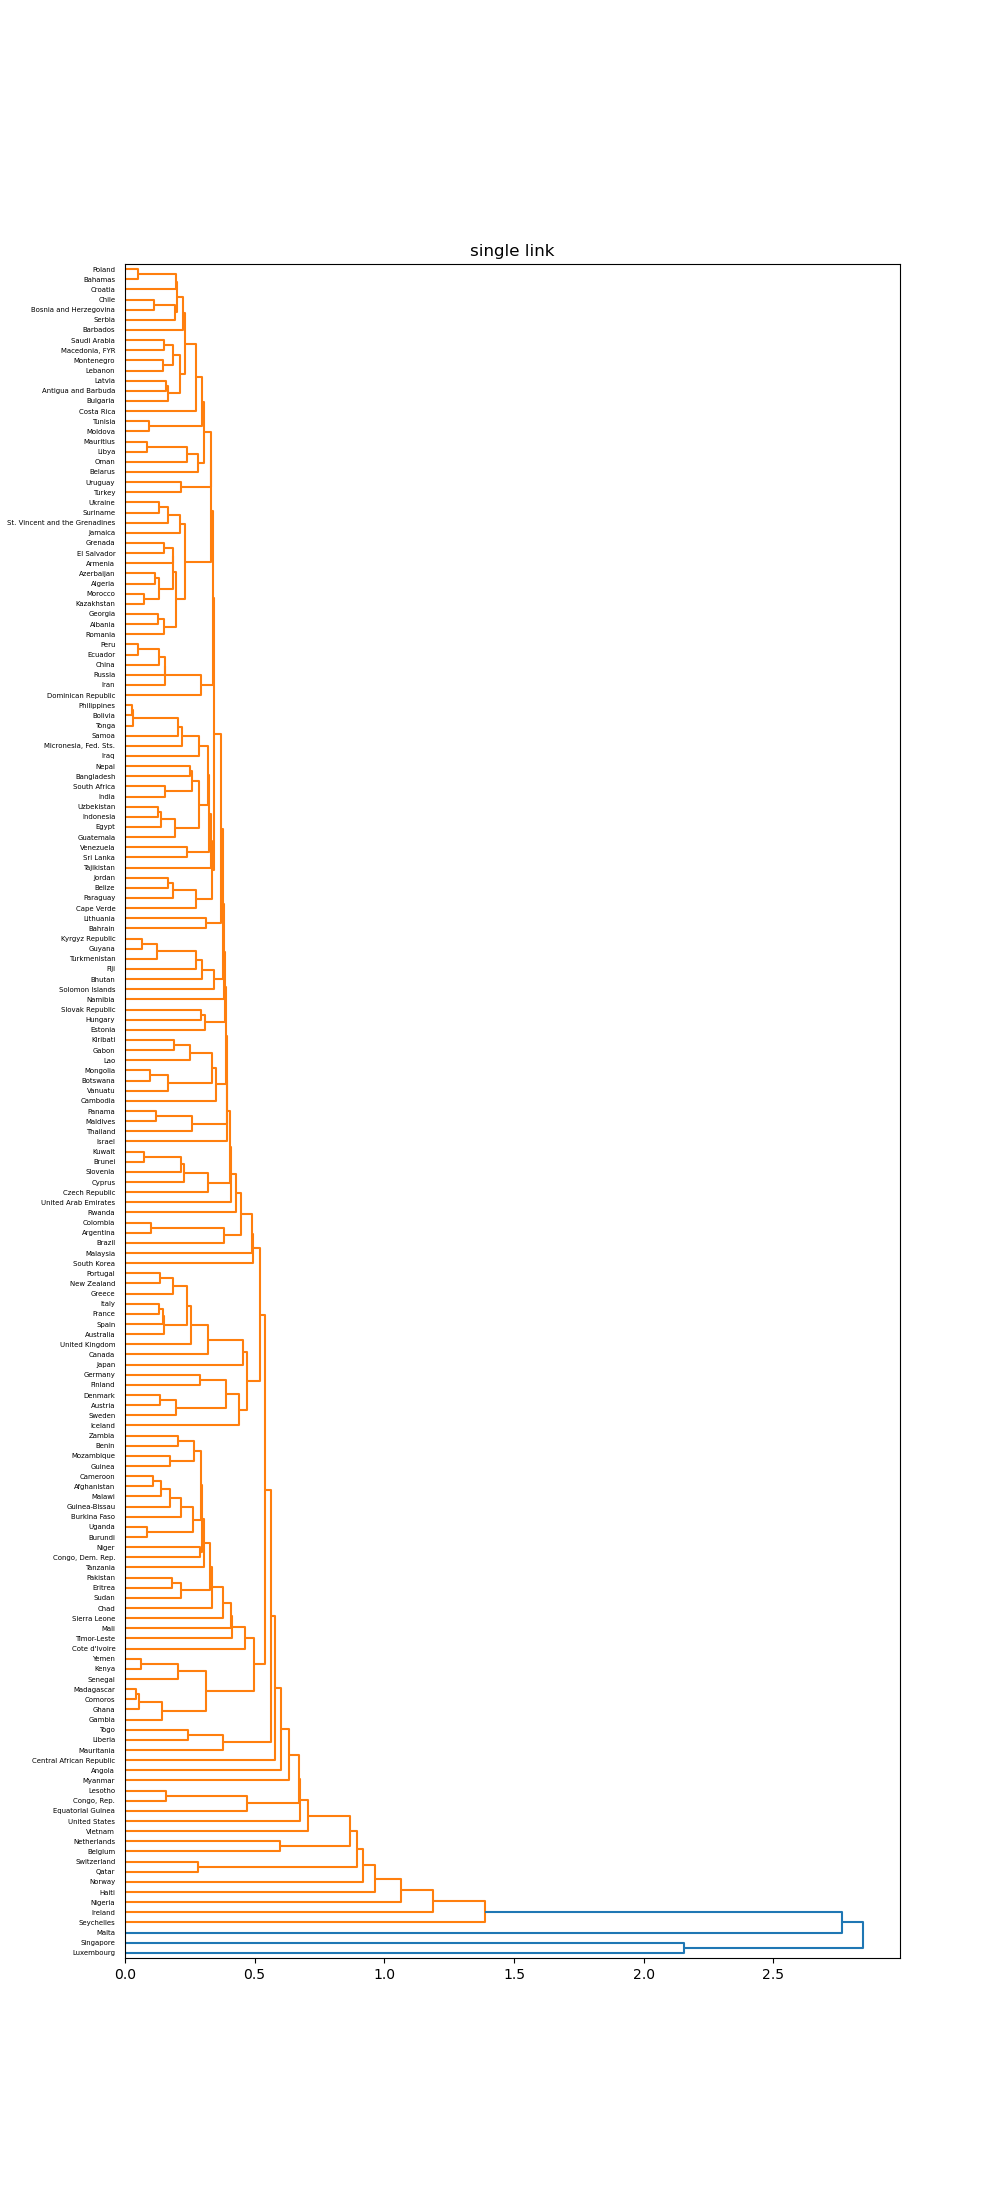
\includegraphics[height=0.93\textheight,trim=0 150 60 165,clip]{s3_single.png}
  \caption{Clustering hiérarchique single link sur \texttt{data\_reduced}.}
  \label{fig:s3-single}
\end{figure}

\begin{figure}[p]
  \centering
  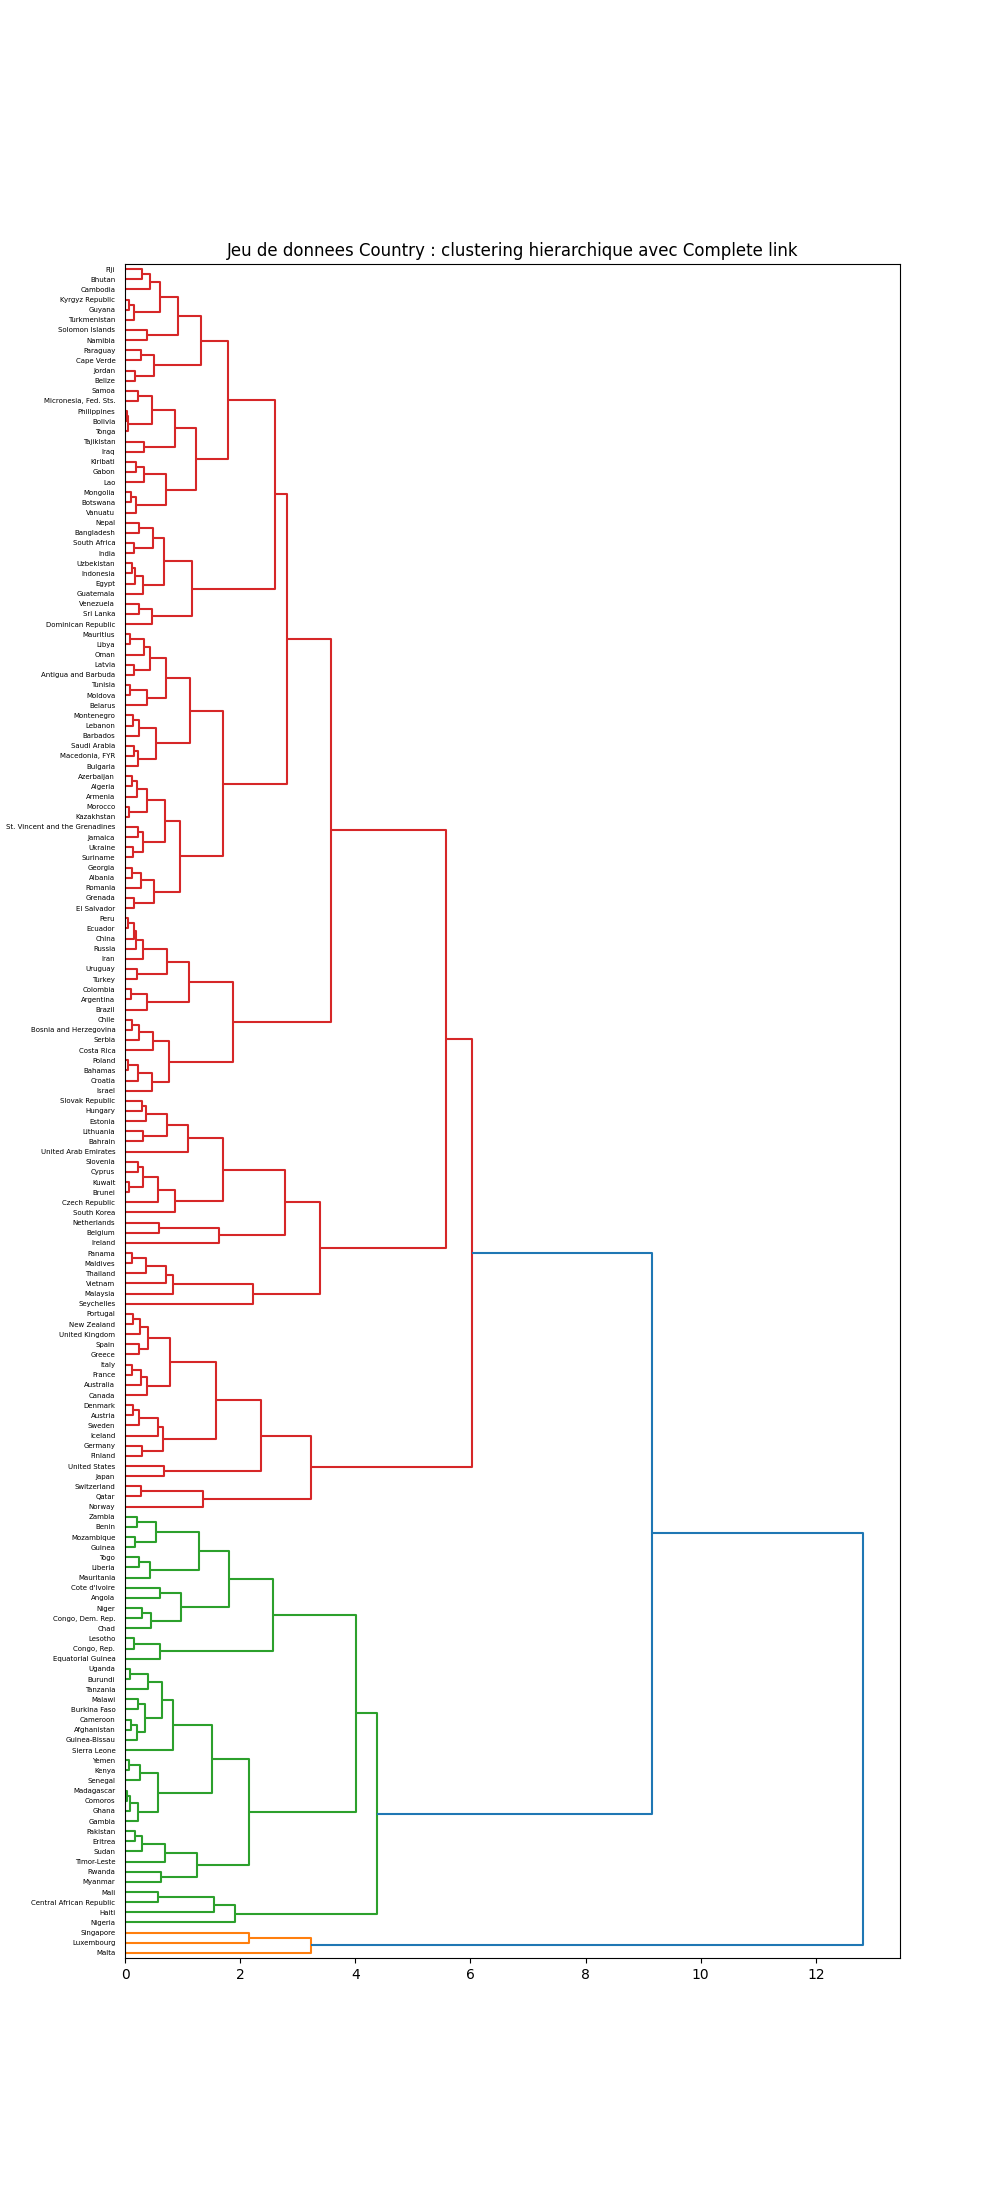
\includegraphics[height=0.93\textheight,trim=0 150 60 165,clip]{s3_complete.png}
  \caption{Clustering hiérarchique complete link sur \texttt{data\_reduced}.}
  \label{fig:s3-complete}
\end{figure}

Pour comparer avec k-means, le script coupe aussi chaque dendrogramme en 2 puis en 3 clusters (\texttt{hierarchy.fcluster}) :
\begin{center}
\begin{tabular}{@{}lccl@{}}
  \toprule
  Méthode & Clusters & Tailles & Petits clusters \\
  \midrule
  Single link   & 2 & 2, 165    & \{Luxembourg, Singapore\} \\
  Single link   & 3 & 2, 164, 1 & \{Luxembourg, Singapore\}, \{Malta\} \\
  Complete link & 2 & 3, 164    & \{Luxembourg, Malta, Singapore\} \\
  Complete link & 3 & 3, 41, 123 & \{Luxembourg, Malta, Singapore\} \\
  \bottomrule
\end{tabular}
\end{center}

\clearpage
\subsubsection*{Interprétation}

\paragraph{Les axes.} Le script affiche la corrélation de chaque variable avec les axes. L'axe X est surtout lié à la mortalité infantile (+0.85), à la fécondité (+0.82), à l'espérance de vie ($-0.87$), au revenu ($-0.81$) et au PIB par habitant ($-0.80$) : il mesure le niveau de développement, les pays pauvres étant à droite. L'axe Y est surtout lié aux importations ($-0.84$) et aux exportations ($-0.76$) en \% du PIB : les pays qui commercent beaucoup avec l'étranger sont en bas.

\paragraph{Équilibre et sens des clusters k-means.} Moyennes de quelques variables dans chaque cluster (affichées par le script) :
\begin{center}
\begin{tabular}{@{}llrrrrrr@{}}
  \toprule
  & Cluster & child\_mort & income & gdpp & life\_expec & total\_fer & exports \\
  \midrule
  $k = 2$ & rouge (89)  & 10.4 & 27\,691 & 22\,216 & 77.0 & 1.9 & 49.9 \\
          & bleu (78)   & 70.1 &  5\,111 &  2\,408 & 63.2 & 4.2 & 31.1 \\
  \midrule
  $k = 3$ & rouge (41)  & 98.6 &  3\,311 &  1\,585 & 59.0 & 5.2 & 28.9 \\
          & orange (78) & 26.2 & 10\,578 &  5\,326 & 71.4 & 2.5 & 35.7 \\
          & bleu (48)   &  6.3 & 39\,631 & 35\,096 & 79.0 & 1.8 & 60.3 \\
  \bottomrule
\end{tabular}
\end{center}
Avec $k = 2$, les clusters sont équilibrés : pays développés ou intermédiaires d'un côté, pays en développement de l'autre. Mais le cluster rouge mélange des pays très différents, comme Norway et Vietnam. Avec $k = 3$, les clusters restent assez équilibrés et correspondent à trois niveaux de développement : pauvre (rouge), intermédiaire (orange) et riche (bleu). C'est le clustering qui nous semble avoir le plus de sens.

\paragraph{Proximité sur la carte du monde.} Pour $k = 3$, les clusters ressemblent à de grandes régions :
\begin{itemize}
  \item rouge : 35 des 41 pays sont en Afrique, les autres sont Afghanistan, Haiti, Lao, Pakistan, Timor-Leste et Yemen ;
  \item bleu : Europe de l'Ouest et du Nord, une partie de l'Europe centrale, United States, Canada, Japan, South Korea, Australia, New Zealand et les pays du Golfe sauf Saudi Arabia ;
  \item orange : presque toute l'Amérique latine, la plupart des pays des Balkans et de l'ex-URSS, l'Afrique du Nord, l'Afrique australe et une grande partie de l'Asie (China, India, Indonesia\dots).
\end{itemize}
La géographie n'entre pas dans le clustering, mais des pays voisins ont souvent un niveau de développement proche. Comme on pouvait s'y attendre, les pays nordiques sont côte à côte sur la Figure~\ref{fig:s3-k3}, tout comme France, Italy et Spain, ou les pays du Sahel (Mali, Niger, Chad). Certaines proximités nous ont surpris :
\begin{itemize}
  \item Haiti est dans le cluster rouge, à côté de Chad et Niger, alors que Dominican Republic, sur la même île, est dans le cluster orange. Dans les données, Haiti a la mortalité infantile la plus élevée (208) et l'espérance de vie la plus faible (32.1 ans) des 167 pays.
  \item Equatorial Guinea et Gabon sont dans le cluster des pays pauvres malgré un revenu élevé (33\,700 et 15\,400), car leur mortalité infantile et leur espérance de vie sont celles des pays pauvres.
  \item Malaysia, Maldives, Panama et Seychelles sont dans le cluster riche avec un PIB par habitant de 7\,100 à 10\,800, alors que Saudi Arabia (19\,300) est dans le cluster orange. Ces quatre pays exportent beaucoup (70 à 94\,\% du PIB), ce qui les place en bas de la figure, plus près du centroïde bleu.
  \item Singapore est très loin de Luxembourg et de Malta sur la carte, mais les trois pays sont proches sur la figure, isolés en bas à gauche. Avec Ireland, ce sont les pays qui exportent le plus (103 à 200\,\% du PIB) : leur proximité vient de leur économie, pas de la géographie.
\end{itemize}

\paragraph{Clusterings hiérarchiques.} En single link, les clusters sont très déséquilibrés (2 et 165 pays) et n'ont pas de sens pour regrouper les pays : à cause de l'effet de chaîne, presque tous les pays sont reliés de proche en proche, et seuls les pays isolés se séparent. Le complete link donne un résultat plus intéressant : en 3 clusters, le cluster de 41 pays a 39 pays en commun avec le cluster rouge de k-means (seuls Myanmar, Rwanda, Gabon et Lao changent). Deux méthodes différentes trouvent donc presque le même groupe de pays pauvres. En revanche, il met ensemble les pays riches et intermédiaires (123 pays) et laisse Luxembourg, Malta et Singapore dans un cluster à part.

\paragraph{Conclusion.} Sur ce jeu de données, k-means avec $k = 3$ donne le clustering le plus utile. Il faut quand même garder en tête que la projection ne garde que 63.1\,\% de la variance, et que l'axe Y rapproche les pays qui commercent beaucoup, quel que soit leur niveau de développement.

\end{document}
